
\section{Applications of Finite Automata}

A finite automaton can be applied to
\begin{compactitem}
\item defining models of computation,
\item testifying equivalence between models,
\item etc.
\end{compactitem}

\begin{definition}[Reverse]
    For a string,
    \[
        \reverse\big( \lst{a_1,a_2,\cdots, a_n} \big) = \lst{a_n, \cdots, a_2, a_1};
    \]
    For a language,
    \[
        \reverse(L) = \set{ \reverse(w) \mid w \in L }.
    \]
\end{definition}

It is easy to find that
\[
    \forall L \in \mathbb R, \reverse (L) \in \mathbb R.
\]

\begin{example}[$\mathbb R$ is closed under union]
    \label{exa:dem_R_closed_under_union}

    Recall \autoref{exa:R_closed_under_union}, with NFA it is much easier to proof the
    theorem now.

    \begin{proof}[Proof of \autoref{exa:R_closed_under_union}]
        Let $M_1, M_2$ be NFAs for $L_1$ and $L_2$,
        build an NFA for $L_1 \cup L_2$
        by simply adding a new initial state that transit to $s_1$ and $s_2$ with
        $\varepsilon$ arrows:
        \centgraph[3cm]{mp/nfa-4.pdf}
    \end{proof}
\end{example}

\begin{example}[$\mathbb R$ is closed under concatenation]
    \begin{proof}
        Let $M_1, M_2$ be NFAs for $L_1$ and $L_2$,
        build an NFA for $L_1 \cdot L_2$:
        \begin{compactenum}
        \item use a new initial state that transit to $s_1$ and $s_2$ with $\varepsilon$
            arrows as in \autoref{exa:dem_R_closed_under_union}; and
        \item change the final states in $M_1$ to regular states and connect them to $s_2$
            with $\varepsilon$ arrows.
        \end{compactenum}
        A rough graph that represents the above steps is
        \begin{center}
            \begin{minipage}{4cm}
                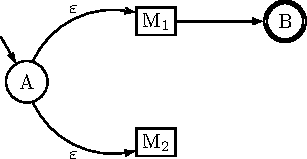
\includegraphics[width=\textwidth]{mp/nfa-5.pdf}
            \end{minipage}
            \; $\longrightarrow$ \;
            \begin{minipage}{4cm}
                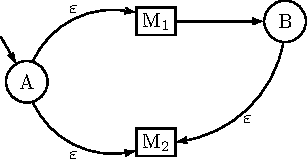
\includegraphics[width=\textwidth]{mp/nfa-6.pdf} 
            \end{minipage}
        \end{center}
        so
        \[
            L(M) = L(M_1) \cdot L(M_2) = \set{ wv \mid w \in L(M_1), v \in L(M_2) }.
        \]
    \end{proof}
\end{example}

